\documentclass[../main.tex]{subfiles}

\begin{document}

\subsubsection*{Methodology}
\subsubsection*{Data analysis}

    \begin{figure}
        \centering
        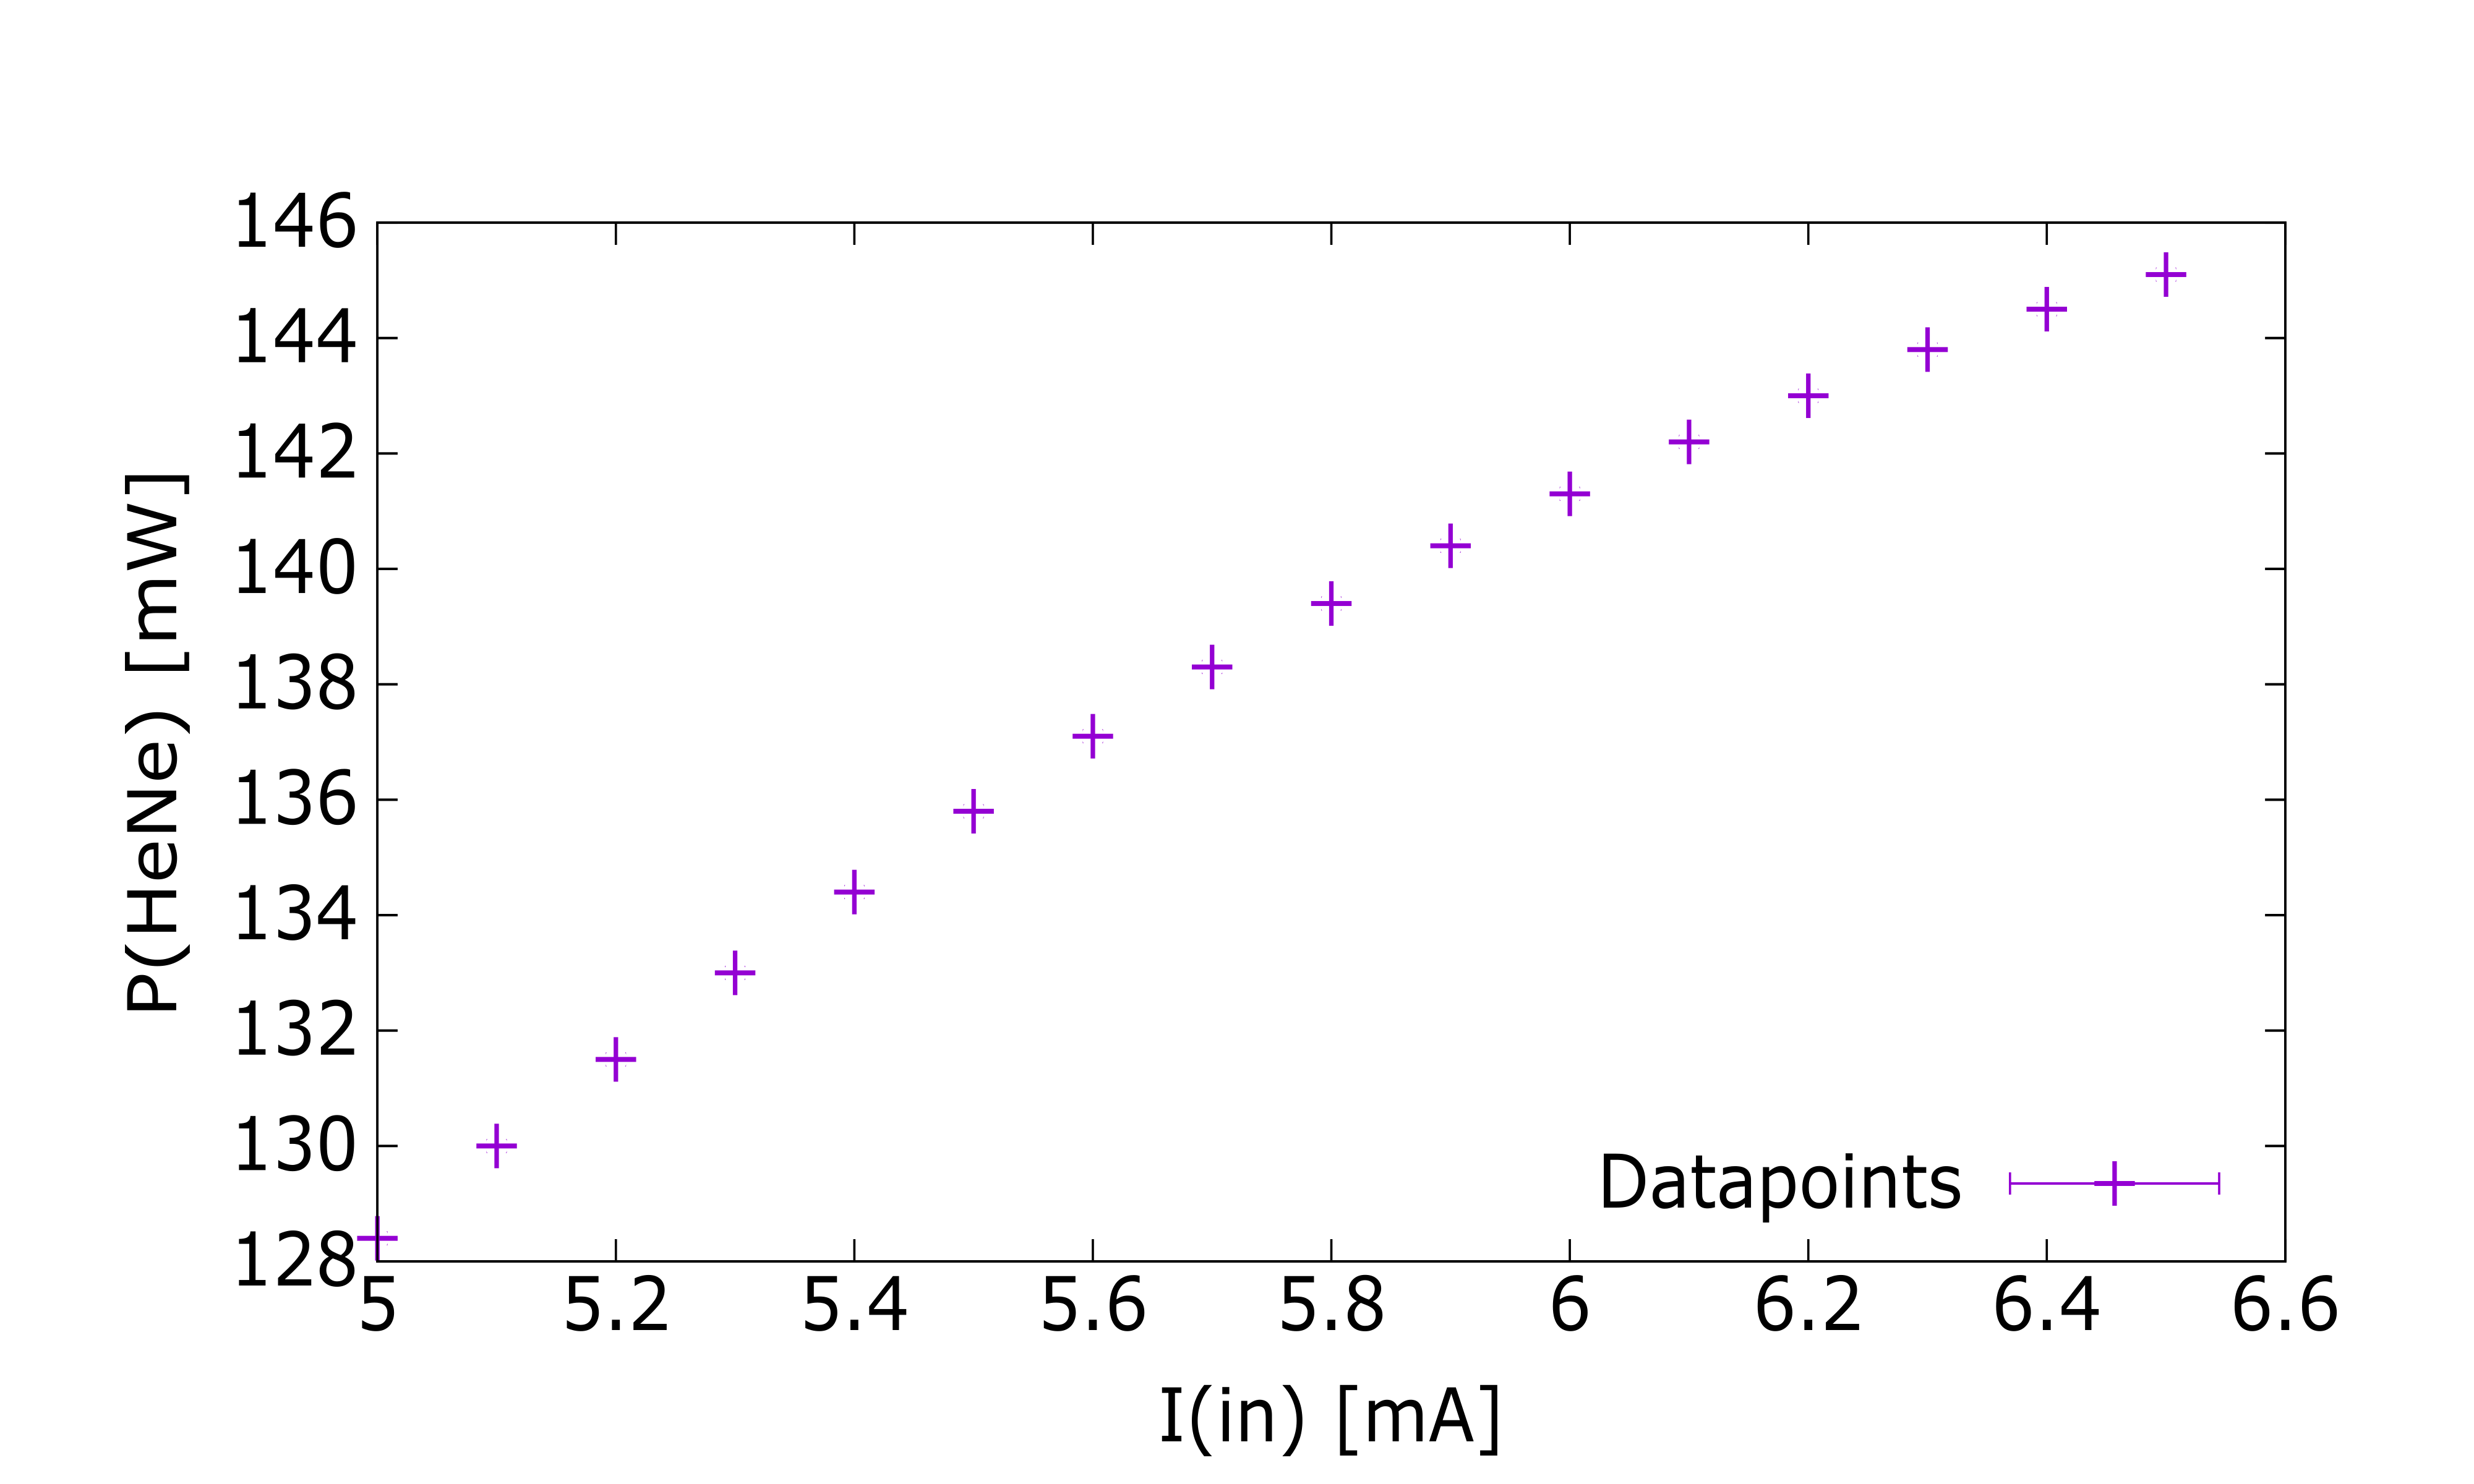
\includegraphics[width=0.8\textwidth]{Bilddateien/6/P(HeNe)overI(in).png}
        \caption{Output power as a function of the input power with the $850\;\si{\mm}$ curved mirror.}
        \label{fig:output_power_over_input_power_curved}
    \end{figure}

    This time we can clearly see a concave nature of the dependency, but we assume the last points to be nearly at the same amplitude which would indicate a saturation in the higher current range. 
\end{document}